\begin{savequote}[75mm] 
Nulla facilisi. In vel sem. Morbi id urna in diam dignissim feugiat. Proin molestie tortor eu velit. Aliquam erat volutpat. Nullam ultrices, diam tempus vulputate egestas, eros pede varius leo.
\qauthor{Quoteauthor Lastname} 
\end{savequote}

\chapter{Results \label{chap5:results}}

This chapter will present the quantitative results of the algorithm described in Chapter \ref{chap4:algorithm} on the software stack presented in Chapter \ref{chap3:architecture}. First, Section \ref{sec:dataset} shows the data used for producing the results. Second, in Section \ref{sec:hardware} the hardware is presented on which the software stack runs. Finally, in Section \ref{sec:results} the tests and the results are presented.

The purpose of this section is to empirically explore the scalability of the algorithm based on input sets.

\section{Data-set \label{sec:dataset}}

The dataset is a synthetic one which is generated beforehand. The input of the algorithm is a $m$ dimensional vector as in Equation \ref{featureVector}.

\begin{equation}
\textbf{x} = [x_{1},\ldots,x_{m}] \in \mathbb{R}^{m} \label{featureVector}
\end{equation}

The value of each feature vector is sampled in a pseudo-random fashion from a Gaussian distribution (also known as the normal distribution), shown in Figure \ref{gaussianDistribution}. The main characteristic of this distribution is that when given a theoretical infinite number of samples, approximately $68.2\%$ of the sampled values are within the $\pm 1$ standard deviation.

\begin{figure}[ht!]
\centering
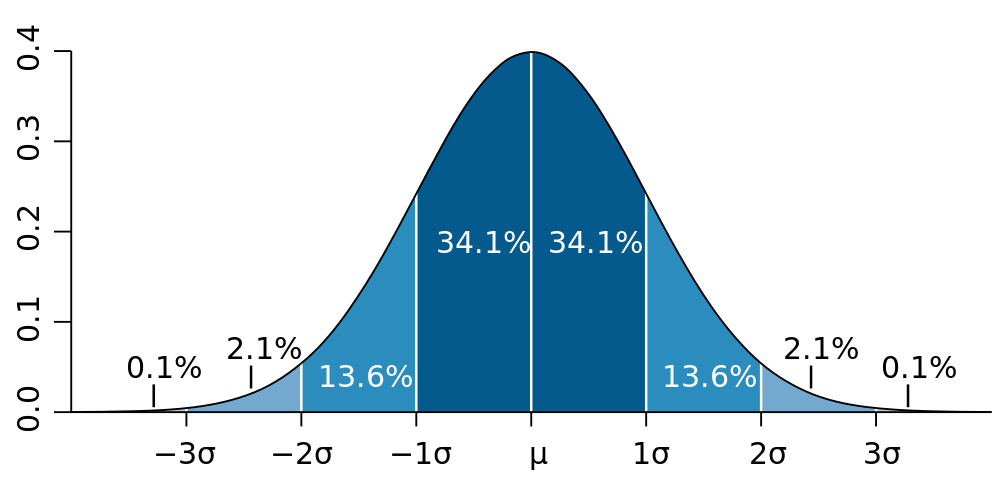
\includegraphics[width=\textwidth]{figures/bellcurve.png}
\caption[Standard normal distribution]{The curve from which the feature vectors are sampled. The vertical axis is the probability. The $\sigma$ values depict the standard deviations. \label{gaussianDistribution}}
\end{figure}

This will result in a dataset where the number of outliers will be limited as the mean of all the observations in the feature space will be at the origin. This will be not a problem as the goal is to determine the scalability of the algorithm and not its performance in determining if the observation is an outlier or not.

\section{Hardware \label{sec:hardware}}
This section will describe the hardware which is used to run the tests. Docker will provide an abstract interface which allows us to run the stack on homogeneous resources. Nevertheless the hardware will impact the actual performance, therefore is it important to describe the hardware: to create an isolated environment which is not affected by other processes running on the physical hardware, a dedicated server has been assigned for running the tests. Quintors' local Dell PowerEdge T620 development-server `Big-Willem' has been assigned for running the algorithm and for producing the results. Big-Willem has two Intel Xeon cpu's with six cores each supporting Hyper-threading, thus providing 24 logical cores in total. The main memory consists of 128 gigabytes in total. 

The virtual machine runs on 16 cores, has 64 gigabytes of memory assigned to it and is fully dedicated to running the software stack.

\section{Results \label{sec:results}}

First, the general execution time as a function of the input size is analyzed in Subsection \ref{subsec:executionTime}. Second, the effect of adding additional workers to the Spark cluster on the exection time is explored in Subsection \ref{subsec:parallelization}. This gives a good insight in the parallelizability of the algorithm. Finally, the stages of the algorithm are defined and insights are given regarding the execution time per stage in Subsection \ref{subsec:shuffle-behaviour}.

\subsection{Execution time \label{subsec:executionTime}}

The total execution time will provide insight of the execution time of the algorithm with a fixed number of resources. The number of observations will be doubled for each iteration starting from $500$ up to $64000$. Every iteration is performed five times to obtain averaged results.
The execution time is given in seconds and is measured after the initialization of the Spark-cluster until the results of the distributed computation are returned to the driver.

\begin{figure}[ht!]
    \begin{center}
        % GNUPLOT: LaTeX picture with Postscript
\begingroup
  \makeatletter
  \providecommand\color[2][]{%
    \GenericError{(gnuplot) \space\space\space\@spaces}{%
      Package color not loaded in conjunction with
      terminal option `colourtext'%
    }{See the gnuplot documentation for explanation.%
    }{Either use 'blacktext' in gnuplot or load the package
      color.sty in LaTeX.}%
    \renewcommand\color[2][]{}%
  }%
  \providecommand\includegraphics[2][]{%
    \GenericError{(gnuplot) \space\space\space\@spaces}{%
      Package graphicx or graphics not loaded%
    }{See the gnuplot documentation for explanation.%
    }{The gnuplot epslatex terminal needs graphicx.sty or graphics.sty.}%
    \renewcommand\includegraphics[2][]{}%
  }%
  \providecommand\rotatebox[2]{#2}%
  \@ifundefined{ifGPcolor}{%
    \newif\ifGPcolor
    \GPcolortrue
  }{}%
  \@ifundefined{ifGPblacktext}{%
    \newif\ifGPblacktext
    \GPblacktexttrue
  }{}%
  % define a \g@addto@macro without @ in the name:
  \let\gplgaddtomacro\g@addto@macro
  % define empty templates for all commands taking text:
  \gdef\gplbacktext{}%
  \gdef\gplfronttext{}%
  \makeatother
  \ifGPblacktext
    % no textcolor at all
    \def\colorrgb#1{}%
    \def\colorgray#1{}%
  \else
    % gray or color?
    \ifGPcolor
      \def\colorrgb#1{\color[rgb]{#1}}%
      \def\colorgray#1{\color[gray]{#1}}%
      \expandafter\def\csname LTw\endcsname{\color{white}}%
      \expandafter\def\csname LTb\endcsname{\color{black}}%
      \expandafter\def\csname LTa\endcsname{\color{black}}%
      \expandafter\def\csname LT0\endcsname{\color[rgb]{1,0,0}}%
      \expandafter\def\csname LT1\endcsname{\color[rgb]{0,1,0}}%
      \expandafter\def\csname LT2\endcsname{\color[rgb]{0,0,1}}%
      \expandafter\def\csname LT3\endcsname{\color[rgb]{1,0,1}}%
      \expandafter\def\csname LT4\endcsname{\color[rgb]{0,1,1}}%
      \expandafter\def\csname LT5\endcsname{\color[rgb]{1,1,0}}%
      \expandafter\def\csname LT6\endcsname{\color[rgb]{0,0,0}}%
      \expandafter\def\csname LT7\endcsname{\color[rgb]{1,0.3,0}}%
      \expandafter\def\csname LT8\endcsname{\color[rgb]{0.5,0.5,0.5}}%
    \else
      % gray
      \def\colorrgb#1{\color{black}}%
      \def\colorgray#1{\color[gray]{#1}}%
      \expandafter\def\csname LTw\endcsname{\color{white}}%
      \expandafter\def\csname LTb\endcsname{\color{black}}%
      \expandafter\def\csname LTa\endcsname{\color{black}}%
      \expandafter\def\csname LT0\endcsname{\color{black}}%
      \expandafter\def\csname LT1\endcsname{\color{black}}%
      \expandafter\def\csname LT2\endcsname{\color{black}}%
      \expandafter\def\csname LT3\endcsname{\color{black}}%
      \expandafter\def\csname LT4\endcsname{\color{black}}%
      \expandafter\def\csname LT5\endcsname{\color{black}}%
      \expandafter\def\csname LT6\endcsname{\color{black}}%
      \expandafter\def\csname LT7\endcsname{\color{black}}%
      \expandafter\def\csname LT8\endcsname{\color{black}}%
    \fi
  \fi
    \setlength{\unitlength}{0.0500bp}%
    \ifx\gptboxheight\undefined%
      \newlength{\gptboxheight}%
      \newlength{\gptboxwidth}%
      \newsavebox{\gptboxtext}%
    \fi%
    \setlength{\fboxrule}{0.5pt}%
    \setlength{\fboxsep}{1pt}%
\begin{picture}(7200.00,5040.00)%
    \gplgaddtomacro\gplbacktext{%
      \csname LTb\endcsname%
      \put(1870,704){\makebox(0,0)[r]{\strut{}$32768$}}%
      \csname LTb\endcsname%
      \put(1870,1074){\makebox(0,0)[r]{\strut{}$65536$}}%
      \csname LTb\endcsname%
      \put(1870,1444){\makebox(0,0)[r]{\strut{}$131072$}}%
      \csname LTb\endcsname%
      \put(1870,1814){\makebox(0,0)[r]{\strut{}$262144$}}%
      \csname LTb\endcsname%
      \put(1870,2184){\makebox(0,0)[r]{\strut{}$524288$}}%
      \csname LTb\endcsname%
      \put(1870,2554){\makebox(0,0)[r]{\strut{}$1.04858\times10^{6}$}}%
      \csname LTb\endcsname%
      \put(1870,2925){\makebox(0,0)[r]{\strut{}$2.09715\times10^{6}$}}%
      \csname LTb\endcsname%
      \put(1870,3295){\makebox(0,0)[r]{\strut{}$4.1943\times10^{6}$}}%
      \csname LTb\endcsname%
      \put(1870,3665){\makebox(0,0)[r]{\strut{}$8.38861\times10^{6}$}}%
      \csname LTb\endcsname%
      \put(1870,4035){\makebox(0,0)[r]{\strut{}$1.67772\times10^{7}$}}%
      \csname LTb\endcsname%
      \put(1870,4405){\makebox(0,0)[r]{\strut{}$3.35544\times10^{7}$}}%
      \csname LTb\endcsname%
      \put(1870,4775){\makebox(0,0)[r]{\strut{}$6.71089\times10^{7}$}}%
      \csname LTb\endcsname%
      \put(2002,484){\makebox(0,0){\strut{}$256$}}%
      \csname LTb\endcsname%
      \put(2602,484){\makebox(0,0){\strut{}$512$}}%
      \csname LTb\endcsname%
      \put(3202,484){\makebox(0,0){\strut{}$1024$}}%
      \csname LTb\endcsname%
      \put(3802,484){\makebox(0,0){\strut{}$2048$}}%
      \csname LTb\endcsname%
      \put(4403,484){\makebox(0,0){\strut{}$4096$}}%
      \csname LTb\endcsname%
      \put(5003,484){\makebox(0,0){\strut{}$8192$}}%
      \csname LTb\endcsname%
      \put(5603,484){\makebox(0,0){\strut{}$16384$}}%
      \csname LTb\endcsname%
      \put(6203,484){\makebox(0,0){\strut{}$32768$}}%
      \csname LTb\endcsname%
      \put(6803,484){\makebox(0,0){\strut{}$65536$}}%
    }%
    \gplgaddtomacro\gplfronttext{%
      \csname LTb\endcsname%
      \put(176,2739){\rotatebox{-270}{\makebox(0,0){\strut{}Execution time in seconds}}}%
      \put(4402,154){\makebox(0,0){\strut{}Samples}}%
    }%
    \gplbacktext
    \put(0,0){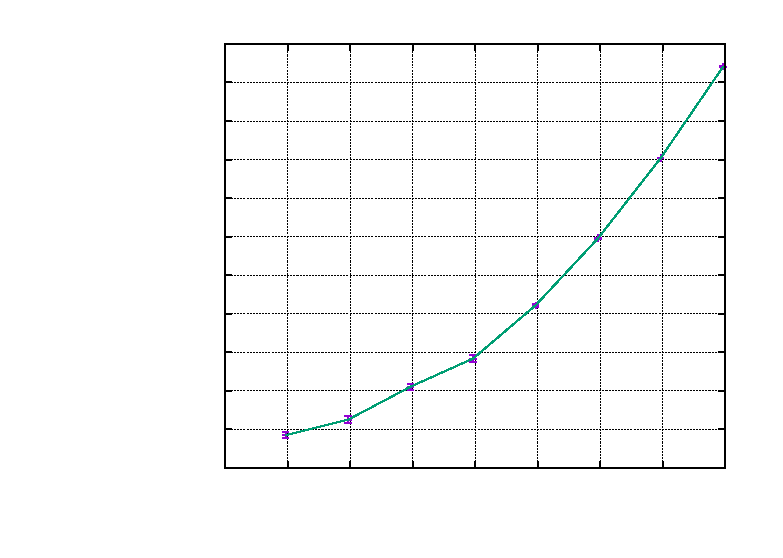
\includegraphics{plots/graph1}}%
    \gplfronttext
  \end{picture}%
\endgroup

    \caption{Execution time as a function of the input size.}
    \label{fig:executiontime}
    \end{center}
\end{figure}

In Figure \ref{fig:executiontime} we observe a quadratic increase in execution time, which is expected as the dominant computational complexity of the algorithm is $\mathcal{O}(n^{2})$ by taking the Cartesian product for computing the distance matrix in Subsection \ref{subsec:distancematrix}.

\subsection{Parallelization \label{subsec:parallelization}}

The purpose of this test is to determine the reduction of execution time by adding additional Spark workers to the cluster. Figure \ref{fig:parallelization} illustrates the execution time as a function of the number of workers.

There will be a single Spark master and a single Apache Zookeeper instance. The number of workers defines the number of Kafka brokers and Spark workers. The number of Kafka nodes is equal to the number of Spark workers since when the number of workers increases, the number of partitions also needs to grow to parallelize the work. Therefore more brokers are desirable to divide the partitions over different brokers.

\begin{figure}[ht!]
    \begin{center}
        % GNUPLOT: LaTeX picture with Postscript
\begingroup
  \makeatletter
  \providecommand\color[2][]{%
    \GenericError{(gnuplot) \space\space\space\@spaces}{%
      Package color not loaded in conjunction with
      terminal option `colourtext'%
    }{See the gnuplot documentation for explanation.%
    }{Either use 'blacktext' in gnuplot or load the package
      color.sty in LaTeX.}%
    \renewcommand\color[2][]{}%
  }%
  \providecommand\includegraphics[2][]{%
    \GenericError{(gnuplot) \space\space\space\@spaces}{%
      Package graphicx or graphics not loaded%
    }{See the gnuplot documentation for explanation.%
    }{The gnuplot epslatex terminal needs graphicx.sty or graphics.sty.}%
    \renewcommand\includegraphics[2][]{}%
  }%
  \providecommand\rotatebox[2]{#2}%
  \@ifundefined{ifGPcolor}{%
    \newif\ifGPcolor
    \GPcolortrue
  }{}%
  \@ifundefined{ifGPblacktext}{%
    \newif\ifGPblacktext
    \GPblacktexttrue
  }{}%
  % define a \g@addto@macro without @ in the name:
  \let\gplgaddtomacro\g@addto@macro
  % define empty templates for all commands taking text:
  \gdef\gplbacktext{}%
  \gdef\gplfronttext{}%
  \makeatother
  \ifGPblacktext
    % no textcolor at all
    \def\colorrgb#1{}%
    \def\colorgray#1{}%
  \else
    % gray or color?
    \ifGPcolor
      \def\colorrgb#1{\color[rgb]{#1}}%
      \def\colorgray#1{\color[gray]{#1}}%
      \expandafter\def\csname LTw\endcsname{\color{white}}%
      \expandafter\def\csname LTb\endcsname{\color{black}}%
      \expandafter\def\csname LTa\endcsname{\color{black}}%
      \expandafter\def\csname LT0\endcsname{\color[rgb]{1,0,0}}%
      \expandafter\def\csname LT1\endcsname{\color[rgb]{0,1,0}}%
      \expandafter\def\csname LT2\endcsname{\color[rgb]{0,0,1}}%
      \expandafter\def\csname LT3\endcsname{\color[rgb]{1,0,1}}%
      \expandafter\def\csname LT4\endcsname{\color[rgb]{0,1,1}}%
      \expandafter\def\csname LT5\endcsname{\color[rgb]{1,1,0}}%
      \expandafter\def\csname LT6\endcsname{\color[rgb]{0,0,0}}%
      \expandafter\def\csname LT7\endcsname{\color[rgb]{1,0.3,0}}%
      \expandafter\def\csname LT8\endcsname{\color[rgb]{0.5,0.5,0.5}}%
    \else
      % gray
      \def\colorrgb#1{\color{black}}%
      \def\colorgray#1{\color[gray]{#1}}%
      \expandafter\def\csname LTw\endcsname{\color{white}}%
      \expandafter\def\csname LTb\endcsname{\color{black}}%
      \expandafter\def\csname LTa\endcsname{\color{black}}%
      \expandafter\def\csname LT0\endcsname{\color{black}}%
      \expandafter\def\csname LT1\endcsname{\color{black}}%
      \expandafter\def\csname LT2\endcsname{\color{black}}%
      \expandafter\def\csname LT3\endcsname{\color{black}}%
      \expandafter\def\csname LT4\endcsname{\color{black}}%
      \expandafter\def\csname LT5\endcsname{\color{black}}%
      \expandafter\def\csname LT6\endcsname{\color{black}}%
      \expandafter\def\csname LT7\endcsname{\color{black}}%
      \expandafter\def\csname LT8\endcsname{\color{black}}%
    \fi
  \fi
    \setlength{\unitlength}{0.0500bp}%
    \ifx\gptboxheight\undefined%
      \newlength{\gptboxheight}%
      \newlength{\gptboxwidth}%
      \newsavebox{\gptboxtext}%
    \fi%
    \setlength{\fboxrule}{0.5pt}%
    \setlength{\fboxsep}{1pt}%
\begin{picture}(7200.00,5040.00)%
    \gplgaddtomacro\gplbacktext{%
      \csname LTb\endcsname%
      \put(1210,704){\makebox(0,0)[r]{\strut{}$65536$}}%
      \csname LTb\endcsname%
      \put(1210,2061){\makebox(0,0)[r]{\strut{}$131072$}}%
      \csname LTb\endcsname%
      \put(1210,3418){\makebox(0,0)[r]{\strut{}$262144$}}%
      \csname LTb\endcsname%
      \put(1210,4775){\makebox(0,0)[r]{\strut{}$524288$}}%
      \csname LTb\endcsname%
      \put(1342,484){\makebox(0,0){\strut{}$0$}}%
      \csname LTb\endcsname%
      \put(1888,484){\makebox(0,0){\strut{}$2$}}%
      \csname LTb\endcsname%
      \put(2434,484){\makebox(0,0){\strut{}$4$}}%
      \csname LTb\endcsname%
      \put(2980,484){\makebox(0,0){\strut{}$6$}}%
      \csname LTb\endcsname%
      \put(3526,484){\makebox(0,0){\strut{}$8$}}%
      \csname LTb\endcsname%
      \put(4073,484){\makebox(0,0){\strut{}$10$}}%
      \csname LTb\endcsname%
      \put(4619,484){\makebox(0,0){\strut{}$12$}}%
      \csname LTb\endcsname%
      \put(5165,484){\makebox(0,0){\strut{}$14$}}%
      \csname LTb\endcsname%
      \put(5711,484){\makebox(0,0){\strut{}$16$}}%
      \csname LTb\endcsname%
      \put(6257,484){\makebox(0,0){\strut{}$18$}}%
      \csname LTb\endcsname%
      \put(6803,484){\makebox(0,0){\strut{}$20$}}%
    }%
    \gplgaddtomacro\gplfronttext{%
      \csname LTb\endcsname%
      \put(176,2739){\rotatebox{-270}{\makebox(0,0){\strut{}Execution time in seconds}}}%
      \put(4072,154){\makebox(0,0){\strut{}Workers}}%
    }%
    \gplbacktext
    \put(0,0){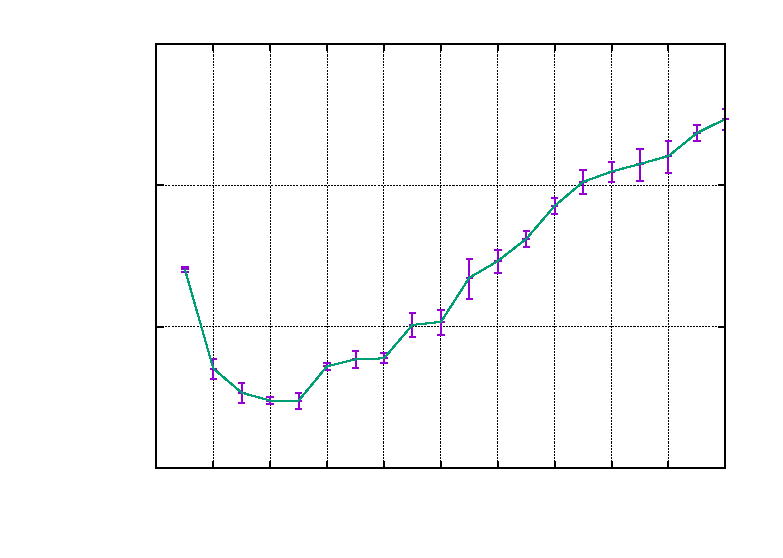
\includegraphics{plots/graph2}}%
    \gplfronttext
  \end{picture}%
\endgroup

        \caption[Execution time as a function of workers.]{Execution time as a function of the number of workers where each worker gets two cores and six gigabytes of RAM assigned, input size $n=2000$, and each worker has three partitions.}
        \label{fig:parallelization}
    \end{center}
\end{figure}

We observe that the execution time decreases until $\text{workers} = 5$, where the cluster works with 10 CPU's and 30 gigabytes of RAM. With the relatively small dataset of $n=2000$, the memory is not a resource constraint. As the machine features 12 physical cores and 24 logical cores, the number of ten cores assigned to Spark is optimal and the number of context-switches will be minimal while utilizing the most resources.

\subsection{Shuffle-behaviour \label{subsec:shuffle-behaviour}}

The shuffle-stages of Apache Spark as introduced in Subsection \ref{subsec_spark} has a major impact on the performance. Especially under big data workloads, this is a known problem \cite{Chen:2009:UTI:1592681.1592693}. At a data-shuffle the RDD, which is scattered across different machines, is distributed from many to many machines. 

Even though moving data is expensive, sometimes it is necessary. For example, certain stages need to consolidate data on a single machine so that it can be co-located in memory to perform computations for the next stage. The algorithm, as proposed in Section \ref{sec:sos}, contains two shuffle stages at:
\begin{description}
  \item[Distance matrix] At the first step, described in Subsection \ref{subsec:distancematrix}, the Cartesian product of the vector input is taken to construct the distance matrix between all pairs.
  \item[Outlier probabilities] The last step takes the product of the matrix, as described in Subsection \ref{subsec:outlierprobabilities}. As all the rows of the matrix are distributed across the different nodes. This requires a shuffle to transfer each row to a single machine to compute the final result. This stage does also includes the binary search to find the affinity for each row, as described in Subsection \ref{subsec:affinity}.
\end{description}

The Cartesian product is first computed using the \texttt{cartesian} primitive, which returns all the pairs of vectors. Then the \texttt{flatmap} primitive is used to compute the distances and remove the diagonal, as it does not hold any information. Last, using \texttt{combineByKey} is used to reduce the pairs to a RDD of vectors which contain the distance from one to another observations.

The intermediate steps, transforming the distance matrix to the affinity matrix in Subsection \ref{subsec:affinity} and computing the binding probability matrix as described in Subsection \ref{subsec:bindingprob} can be done locally on each worker for each vector in the RDD.

Lastly, the position of the value in the vector is assigned a key and the final result is computed using \texttt{foldLeft} which requires a shuffle as the rows of the matrix are local, and the columns are distributed across multiple machines.

Using the Spark Event Log\footnote{Spark monitoring \url{http://spark.apache.org/docs/latest/monitoring.html}}, the time taken for each stage can be monitored. This information is helpful to obtain insights about the bottlenecks of the algorithm.

\begin{table}[ht!]
\makebox[\linewidth]{
\centering

\begin{tabular}{r|llll|llll|llll}
 ~ & \multicolumn{4}{c|}{$N=2400$} & \multicolumn{4}{c|}{$N=4800$} & \multicolumn{4}{c}{$N=9600$}\\
 ~ & Distance & Product & Collect & Sum & Distance & Product & Collect & Sum & Distance & Product & Collect & Sum \\ \hline
 Run 1 & 114 & 90 & 6 & 210 & 258 & 330 & 6 & 594 & 900 & 1380 & 9 & 2289 \\
 Run 2 & 114 & 90 & 6 & 210 & 252 & 330 & 6 & 588 & 780 & 1380 & 12 & 2172 \\
 Run 3 & 114 & 90 & 6 & 210 & 258 & 330 & 6 & 594 & 900 & 1380 & 10 & 2290 \\
 Run 4 & 114 & 90 & 6 & 210 & 282 & 330 & 6 & 618 & 1080 & 1380 & 8 & 2468 \\
 Run 5 & 108 & 102 & 6 & 216 & 264 & 330 & 6 & 660 & 1260 & 1380 & 9 & 2649 \\
 Run 6 & 114 & 90 & 6 &	210 & 270 & 402 & 5 & 677 & 1080 & 1380 & 11 & 2471 \\
 Run 7 & 126 & 84 & 6 & 216 & 252 & 330 & 6 & 588 & 1320 & 1380 & 12 & 2712 \\
 Run 8 & 144 & 90 & 6 & 240 & 276 & 402 & 5 & 683 & 960 & 1380 & 12 & 2352 \\
 Run 9 & 138 & 102 & 6 & 246 & 270 & 330 & 5 & 605 & 900 & 1380 & 11 & 2291 \\
 Run 10 & 114 & 102 & 5 & 221 & 258 & 342 & 6 & 606 & 960 & 1380 & 11 & 2351 \\
 Average & 120.00 & 93.00 & 5.9 & 218.9 & 5.7 & 345.6 & 264 & 615.3 & 1014 & 1380 & 10.5 & 2404.5 \\
 Std.dev & 12.00 & 6.48 & 0.32 & 13.32 & 0.48 & 29.96 & 10.2 & 35.31 & 170.76 & 0 & 1.43 & 177.56 \\ \hline
 Total & 42.49\% & 54.82\% & 2.70\% & ~ & 42.91\% & 56.17\% & 0.92\% & ~ & 42.17\% & 57.39\% & 0.43\% & ~ \\
\end{tabular}
}
\caption[Execution time taken per stage]{Time taken for each stage of the algorithm execution. The distance column refers to the Cartesian product of the vectors to compute the distance-matrix. The product column refers to the shuffle required to consolidate each column of the matrix on a single worker. The collect column is the time taken to bring the results back to the driver. Everything is in seconds.}

\label{table:executionPerStage}

\end{table}

Table \ref{table:executionPerStage} provides insights in the execution time per stage. Each stage is delimited by a shuffle at which the different worker nodes in the cluster have to coordinate and transfer the data which is required for the next stage. We observe that the last stage, which entails the binary search and the shuffling of the columns, covers the majority of the execution time. At first glance the Cartesian product is likely to be the dominant factor, but the share of this stage decreases as the number of observations grows.

